\ylDisplay{Küttekeha} % Ülesande nimi
{Tundmatu autor} % Autor
{lõppvoor} % Voor
{2012} % Aasta
{P 6} % Ülesande nr.
{2} % Raskustase
{
% Teema: Elektriõpetus

\ifStatement
Juku tahab endale ehitada võimalikult võimsat veekeetjat. Selleks on tal küttekeha alusplaat, millele saab ühendada takisteid nagu näidatud joonisel, ja $4$ takistit, mille takistused on $30$ $\Omega$, $20$ $\Omega$, $15$ $\Omega$ ja $10$ $\Omega$. Kuidas peaks ta takistid plaadil olevatesse pesadesse paigutama, et saavutada maksimaalne võimsus, kui seadet toidetakse pingega $230$ V, ja pinge rakendatakse kontaktide $A$ ja $B$ vahele? Kui suur on see maksimaalne võimsus?
\begin{center}
	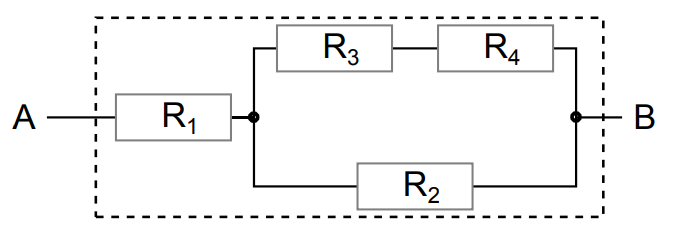
\includegraphics[width=0.5\linewidth]{2012-v3p-06-yl.png}
\end{center}
\fi

\ifHint
Maksimaalse võimsuse jaoks takistus minimeerida.
\fi

\ifSolution
Võimsus konstantse pingeallika korral on $P = U I = U^2 / R$. Seega tuleb maksimaalse võimsuse jaoks takistus minimeerida. Ahelda takistus on leitav kui:
\begin{center}
$R = R_1 + \frac{1}{\cfrac{1}{R_2} + \cfrac{1}{R_3 + R_4}}$.
\end{center}
Parim kombinatsioon on: $R_1 = 10$ $\Omega$, $R_2 = 15$ $\Omega$, $R_3 = 20$ $\Omega$ ja $R_4 =30 \Omega$.
Selle korral on takistuseks $R \approx 21,5$ $\Omega$ ja võimsus $P \approx 2,46 k$.
\fi
}